\documentclass[handout]{beamer}
\mode<presentation>
{
  \usetheme{Warsaw}
  \definecolor{mcgarnet}{rgb}{0.38, 0, 0.08}
  \definecolor{mcgray}{rgb}{0.6, 0.6, 0.6}
  \setbeamercolor{structure}{fg=mcgarnet,bg=mcgray}
  %\setbeamercovered{transparent}
}


\usepackage[english]{babel}
\usepackage[latin1]{inputenc}
\usepackage{times}
\usepackage[T1]{fontenc}
\usepackage{tikz}
\usepackage{graphicx}
\usepackage{adjustbox}
\usepackage{fancyvrb}

\newcommand{\imagesource}[1]{{\centering\hfill\break\hbox{\scriptsize Image Source:\thinspace{\small\itshape #1}}\par}}

\title{(Re)Introduction to C++}


\author{Dr. Robert Lowe\\}

\institute[Maryville College] % (optional, but mostly needed)
{
  Division of Mathematics and Computer Science\\
  Maryville College
}

\date[]{}
\subject{}

\pgfdeclareimage[height=0.5cm]{university-logo}{images/Maryville-College}
\logo{\pgfuseimage{university-logo}}



\AtBeginSection[]
{
  \begin{frame}<beamer>{Outline}
    \tableofcontents[currentsection]
  \end{frame}
}


\begin{document}

\begin{frame}
  \titlepage
\end{frame}

\begin{frame}{Outline}
  \tableofcontents
\end{frame}


% Structuring a talk is a difficult task and the following structure
% may not be suitable. Here are some rules that apply for this
% solution: 

% - Exactly two or three sections (other than the summary).
% - At *most* three subsections per section.
% - Talk about 30s to 2min per frame. So there should be between about
%   15 and 30 frames, all told.

% - A conference audience is likely to know very little of what you
%   are going to talk about. So *simplify*!
% - In a 20min talk, getting the main ideas across is hard
%   enough. Leave out details, even if it means being less precise than
%   you think necessary.
% - If you omit details that are vital to the proof/implementation,
%   just say so once. Everybody will be happy with that.

\section{C++ Basics}

\begin{frame}[fragile]{Structure of a C++ Program}
\begin{verbatim}
// File: boilerplate.cpp
// Purpose: Sample C++ Program
// Author: Your Name Here
#include <iostream>

using namespace std;

int main()
{

}
\end{verbatim}
\end{frame}

\begin{frame}[fragile]{Compiling C++ Programs}
    \begin{itemize}
        \item \verb!g++ program.cpp -o program!
        \item \verb!make program!
    \end{itemize}
\end{frame}

\begin{frame}{Variables}
    \begin{itemize}
        \item Variables are named areas of memory.
        \item In C++, variables must be declared before they can be
            used.
        \item A variable declaration has the form:
            \newline\texttt{type} \texttt{identifier}
        \item Identifiers consist of letters, numbers, and
            underscores.
        \item Identifiers must begin with a letter or underscore.
        \item Words in variable names are usually separated by
            underscores, or via camleCasing.
    \end{itemize}
\end{frame}

\begin{frame}{Data Types}
    \begin{block}{Primitive Data Types}
        \begin{description}
            \item[\texttt{char}] - Character, single letter/symbol
            \item[\texttt{bool}] - Boolean true or false value
            \item[\texttt{int}] - Integer (whole number)
            \item[\texttt{float}] - Single precision floating point
                number (never use!)
        \end{description}
    \end{block}

    \begin{block}{Common Complex Types}
        \begin{description}
            \item[\texttt{string}] - A string of characters
            \item[\texttt{ifstream}] - An input file stream (for reading)
            \item[\texttt{ofstream}] - An output file stream (for
                writing)
            \item[\texttt{vector<type>}] - A list of variables of
                \texttt{type}.
        \end{description}
    \end{block}
\end{frame}

\begin{frame}[fragile]{Input and Output}
    \begin{itemize}
        \item Input is accomplished via the extraction operator:
            \newline\texttt{cin >> x;}
        \item Output is accomplished via the insertion operator:
            \newline\texttt{cout << "Hello, World" << endl;}
            \newline\texttt{cout << x << endl;}
    \end{itemize}
\end{frame}

\begin{frame}[fragile]{Programming Project P1.2}
    From the end of chapter 1 in \textit{Big C++}:

    \begin{block}{Programming Problem P1.2}
    Write a program that prints out a message ``Hello, my name is
    Hal!''
    Then, on a new line, the program should print the message ``What is
    your name?'' As in Exercise P1.1, just use the following lines of
    code:

    \begin{verbatim}
        string user_name;
        getline(cin, user_name);
    \end{verbatim}

    Finally, the program should print the message ``Hello, user name.
    I am glad to meet you!'' 
    \end{block}
\end{frame}

\section{Operations and Decisions}

\begin{frame}[fragile]{Operator Precedence (thus far)}
  \begin{adjustbox}{max totalheight=0.8\textheight}
    \begin{tabular}{|l|l|l|}
        \hline
        \textbf{Operator} & \textbf{Description} & \textbf{Associativity} \\
        \hline
        \texttt{a++}, \verb#a--# & Postfix increment and decrement & Left-to-Right\\
        \hline
        \texttt{not}, \texttt{!} & Logical Not & Right-to-Left\\
        \texttt{++a}, \verb#--a# & Prefix increment and decrement &  \\
        \hline
        \texttt{a*b}, \texttt{a/b}, \texttt{a\%b} & Multiply, Divide, Modulus & Left-to-Right\\
        \hline
        \texttt{a+b}, \texttt{a-b} & Addition and Subtraction & Left-to-Right\\
        \hline
        \texttt{<<} , \texttt{>>} & Insertion and Extraction & Left-to-Right \\
        \hline
        \texttt{<}, \texttt{<=} & Relational Operators & Left-to-Right\\
        \texttt{>}, \texttt{>=} & & \\
        \hline
        \texttt{==}, \texttt{!=} & Equality Operators & Left-to-Right\\
        \hline
        \texttt{and}, \texttt{\&\&} & Logical And & Left-to-Right\\
        \hline
        \texttt{or}, \texttt{||} & Logical Or & Left-to-Right\\
        \hline
        \texttt{=},  & Assignment and Assignment & Right-to-Left \\
        \texttt{+=}, \texttt{-=} & & \\
        \texttt{*=}, \texttt{/=} & & \\
        \texttt{\%=} & & \\
        \hline
    \end{tabular}
  \end{adjustbox}
\end{frame}

\begin{frame}[fragile]{If Statement}
\begin{columns}
    \column{0.5\textwidth}
    \verb!if(! \textit{condition} \verb!)! 
    \verb!    ! \textit{statement/block}

    \vspace{2cm}

    \begin{itemize}[<+(1)->]
        \item If the \textit{condition} is true, the
            \textit{statement/block} will be executed.
        \item If the \textit{condition} is false, the 
            \textit{statement/block} will be skipped.
    \end{itemize}

    \column{0.5\textwidth}
    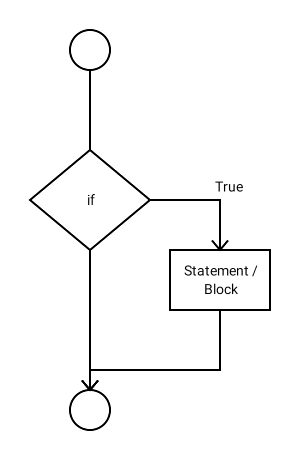
\includegraphics[width=0.9\textwidth]{images/if}
\end{columns}
\end{frame}

\begin{frame}[fragile]{If Else Statement}
\begin{columns}
    \column{0.5\textwidth}
    \verb!if(! \textit{condition} \verb!)! 
    \newline\verb!    ! \textit{then statement/block}
    \newline\verb!else!
    \newline\verb!    ! \textit{else statement/block}

    \vspace{1cm}

    \begin{itemize}[<+(1)->]
        \item If the \textit{condition} is true, the
            \textit{then statement/block} will be executed.
        \item If the \textit{condition} is false, the 
            \textit{else statement/block} will be executed.
    \end{itemize}

    \column{0.5\textwidth}
    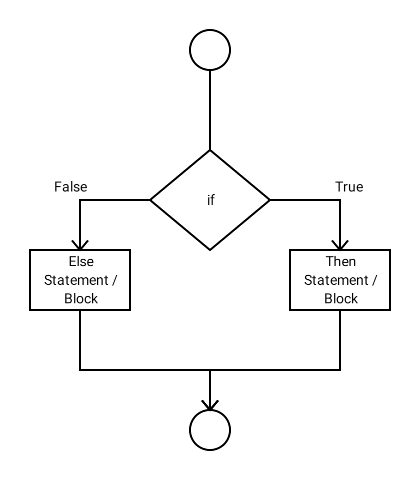
\includegraphics[width=0.9\textwidth]{images/if-else}
\end{columns}
\end{frame}

\begin{frame}[fragile]{Multi-Way Branching: If-Then-Else-If}
\begin{columns}
    \column{0.5\textwidth}
    \verb!if(! \textit{condition} \verb!)! 
    \newline\verb!    ! \textit{then statement/block}
    \verb!else if(! \textit{condition} \verb!)! 
    \newline\verb!    ! \textit{then statement/block}
    \newline\verb!else!
    \newline\verb!    ! \textit{else statement/block}
    
    \vspace{0.5cm}

    \begin{itemize}[<+(1)->]
        \item The first then \textit{statement/block} with a true condition executes.
        \item If no matches are found, the (optional) \textit{else statement/block} executes.
    \end{itemize}

    \column{0.5\textwidth}
    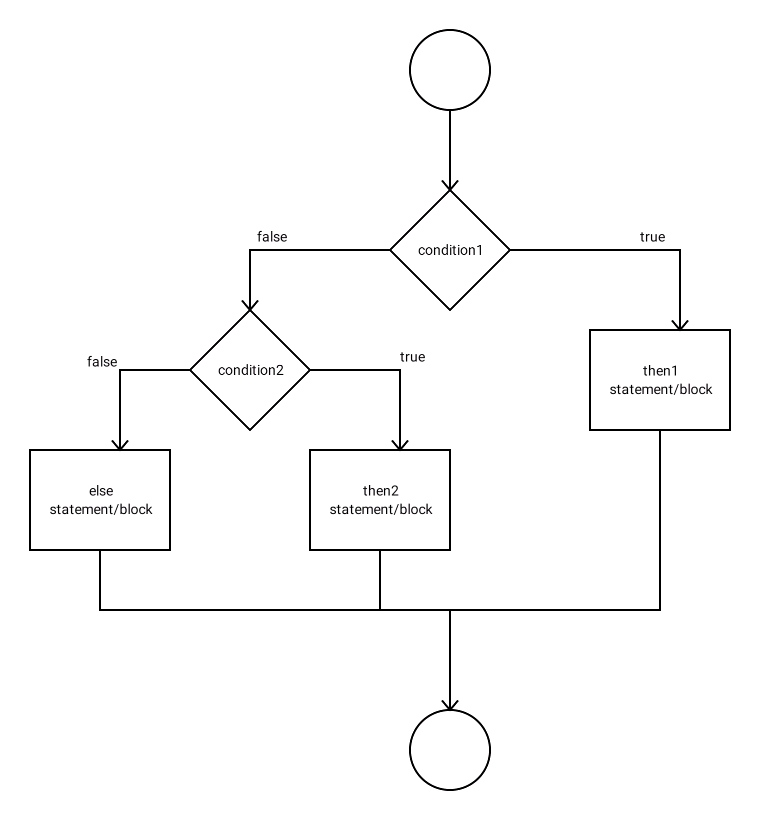
\includegraphics[width=0.9\textwidth]{images/if-elseif}
\end{columns}
\end{frame}

\begin{frame}[fragile]{Programming Project P3.3}
    From the end of Chapter 3 in \textit{Big C++}:

    \begin{block}{Programming Problem P3.3}
    Write a program that takes user input describing a playing card in the following shorthand notation:
    \newline A Ace
    \newline 2 ... 10  Card values
    \newline J Jack
    \newline Q Queen
    \newline K King
    \newline D Diamonds
    \newline H Hearts
    \newline S Spades
    \newline C Clubs

    Your program should print the full description of the card. 
    \end{block}
\end{frame}

\end{document}


